\documentclass[12pt,a4paper,titlepage]{article}
\usepackage[left=2.5cm,text={16cm,20cm},top=4cm]{geometry}
\usepackage[T1]{fontenc}
\usepackage[czech]{babel}
\usepackage[utf8]{inputenc}
% dalsi balicky
\usepackage{graphicx}
\usepackage{enumitem}
\usepackage{indentfirst}
\usepackage{float}
\usepackage{svg}
\usepackage{amsmath}
\usepackage{url}
\usepackage{graphics}
\usepackage{graphicx}
\usepackage{multicol}
\graphicspath{ {images/} }
\usepackage[bookmarksopen,colorlinks,plainpages=false,urlcolor=blue,
unicode,linkcolor=black]{hyperref}

\bibliographystyle{czplain}

%úvodzovky
\providecommand{\uv}[1]{\quotedblbase #1\textquotedblleft}

\begin{document}

\begin{titlepage}
\begin{center}
    {
    	\Huge\textsc{Vysoké učení technické v~Brně}}\\
    \smallskip
    {
    	\huge\textsc{Fakulta informačních technologií}}\\
    \bigskip
    \vspace{\stretch{0.382}} %pomery odpovedajúcí zlatému rezu    
    \huge{Pokročilé databázové systémy}\\
    \smallskip
    \Huge{Projekt -- map maker}\\
    \vspace{\stretch{0.618}}
\end{center}
    {\Large \today \hfill David Kozák (xkozak15)  }\\
    \smallskip
    {\Large \hfill Pavel Plaskoň (xplask00)  }\\
    \smallskip
    {\Large \hfill Jan Velecký (xvelec07)  }\\
\end{titlepage}

\newpage
\tableofcontents
\newpage

\section{Úvod}

\section{Přeložení a spuštění aplikace}

\section{Popis grafického uživatelského rozhraní}

\begin{figure}[!htbp]
	\centering
	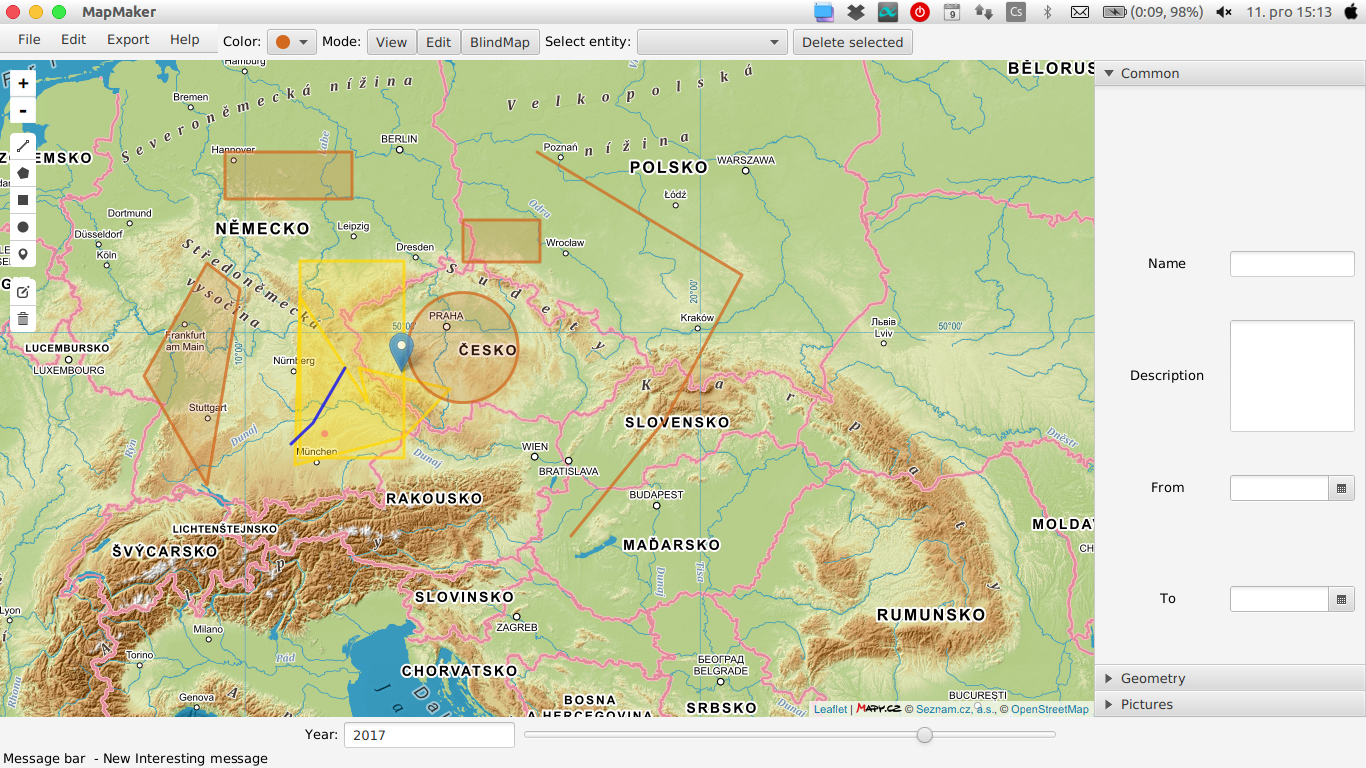
\includegraphics[scale=0.3]{full_window}
	\caption{Celé okno}
	\label{fullWindow}
\end{figure}

\subsection{Hlavní okno}

\subsection{Pravá lišta}

\begin{figure}[!htbp]
	\centering
	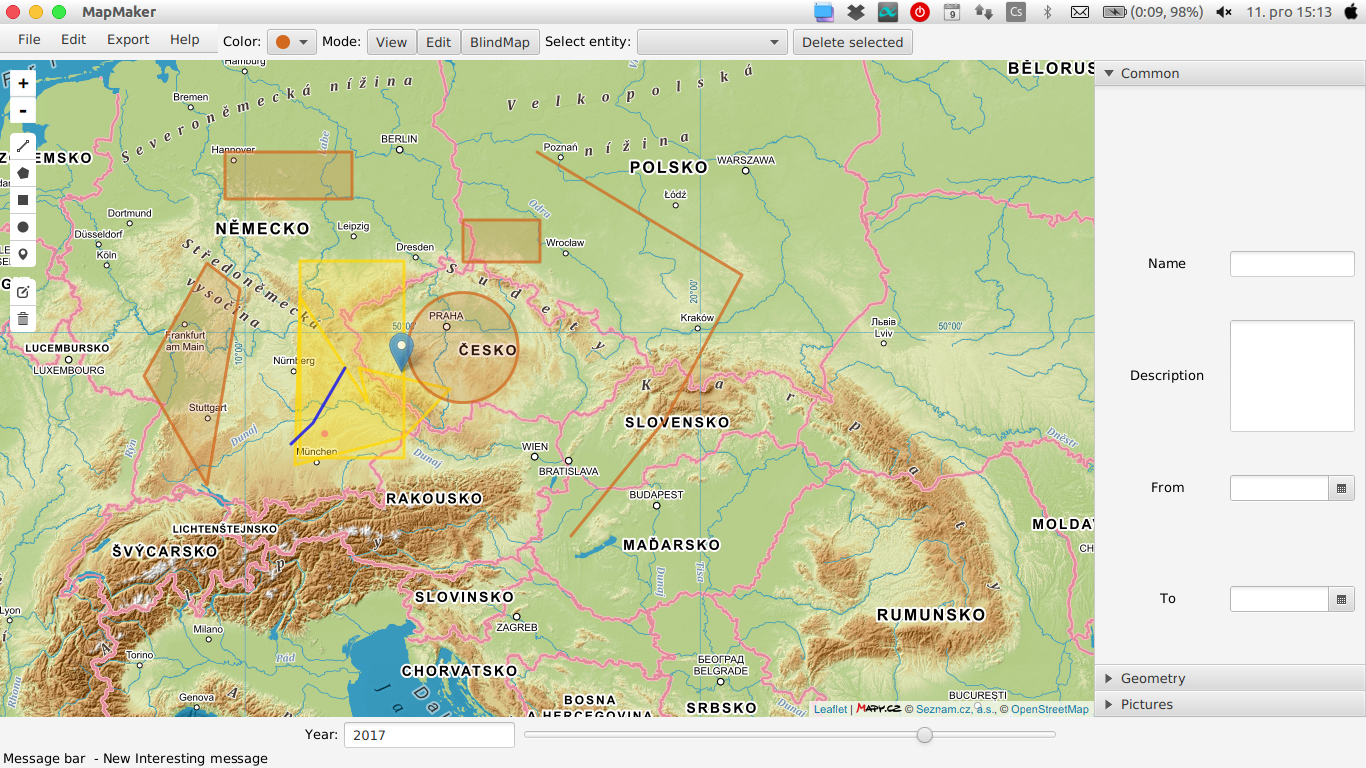
\includegraphics[scale=0.25]{full_window}
	\caption{Details pravá lišta}
	\label{rightBar}
\end{figure}

\subsection{Slepá mapa}

\begin{figure}[!htbp]
	\centering
	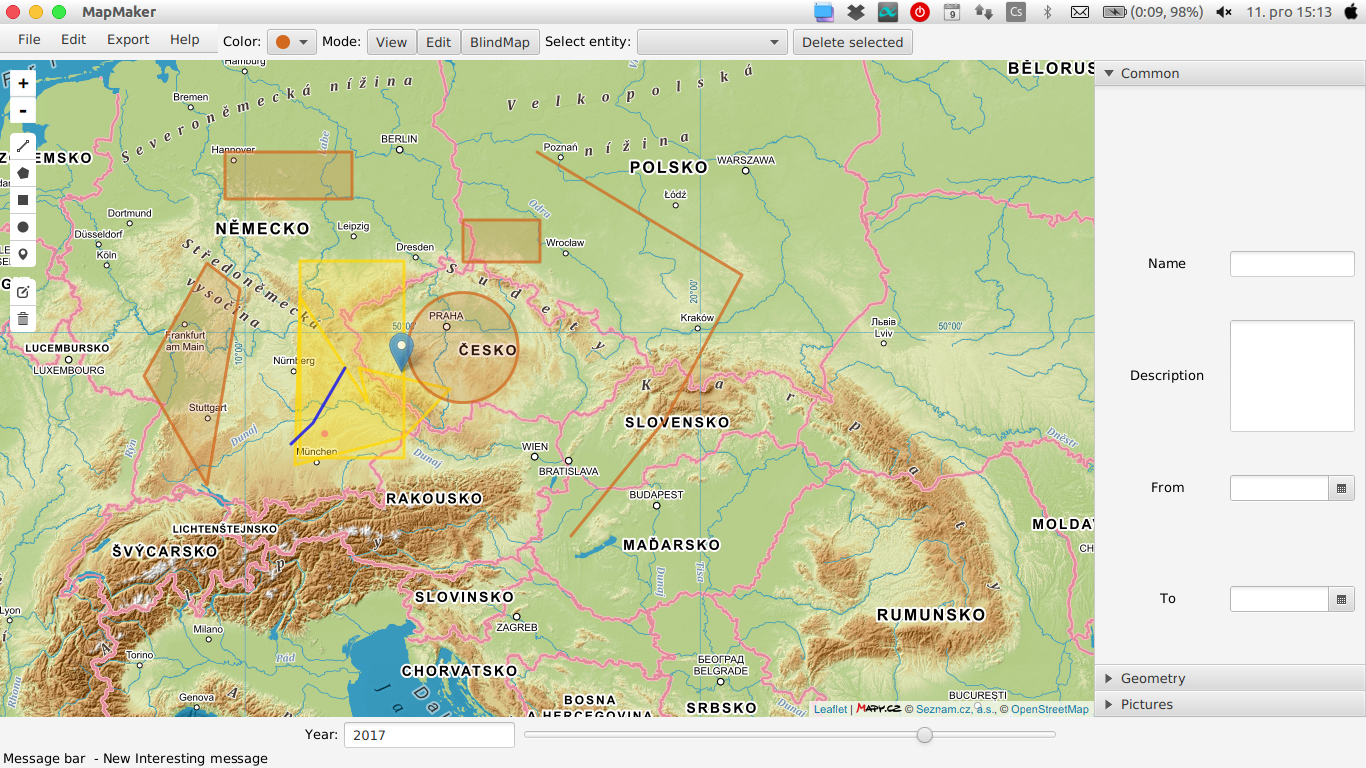
\includegraphics[scale=0.25]{full_window}
	\caption{Detail slepá mapa}
	\label{blindMap}
\end{figure}

\subsection{Nastavení}
\begin{figure}[!htbp]
	\centering
	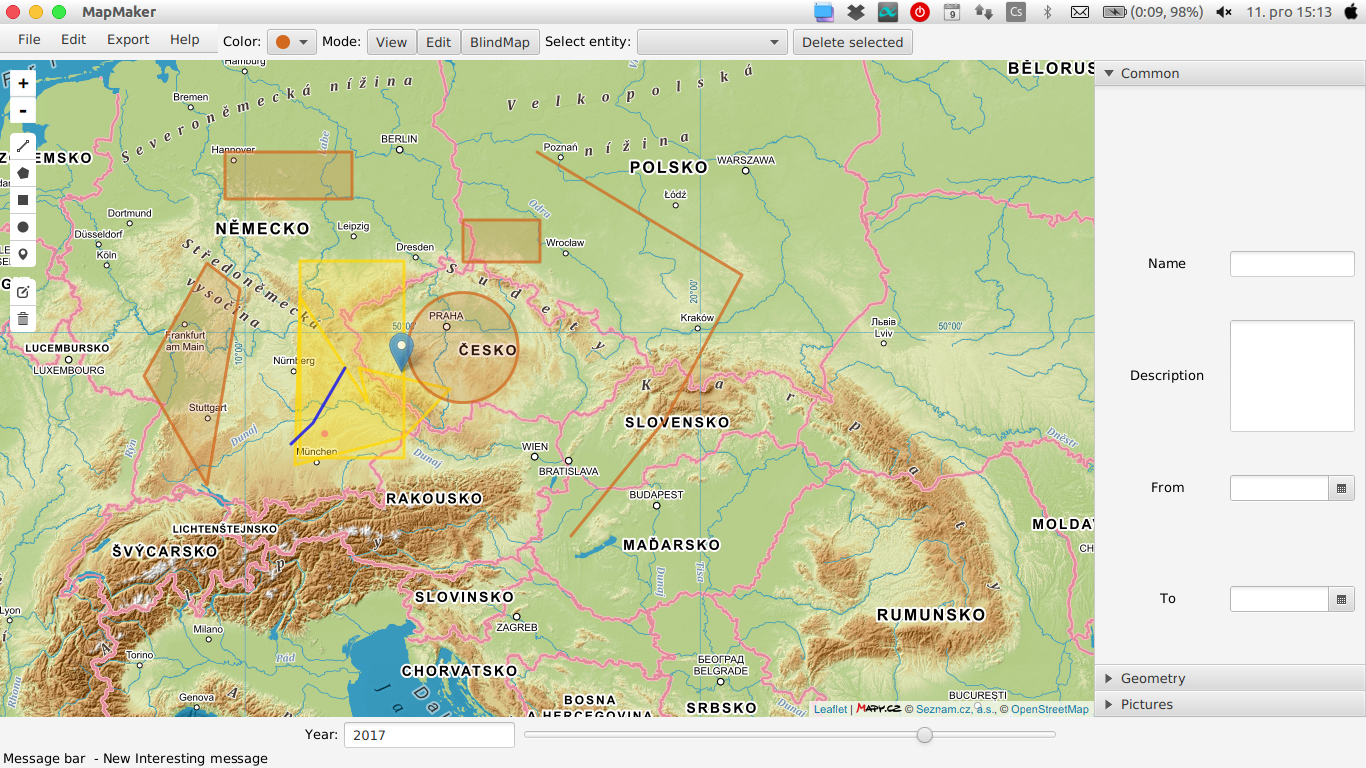
\includegraphics[scale=0.25]{full_window}
	\caption{Details nastavení}
	\label{settings}
\end{figure}

\section{Prostorové dotazy}

\subsection{Složité dotazy}

\subsection{Analytické funkce}

\end{document}